% Memoria de la Práctica 4 - Metodología de la Programación Paralela
% CUDA Programming
\documentclass[12pt,a4paper]{report}

% -------------------- Configuración y Paquetes --------------------
\usepackage[utf8]{inputenc}
\usepackage[T1]{fontenc}
\usepackage[spanish,es-tabla]{babel} % es-tabla usa "Tabla" en lugar de "Cuadro"
\usepackage{geometry}
\geometry{left=3cm,right=2.5cm,top=3cm,bottom=3cm}
\usepackage[protrusion=true,expansion=false]{microtype}

% Figuras y Gráficos
\usepackage{graphicx}
\usepackage{float}
\usepackage{caption}
\usepackage{subcaption}

% Tablas
\usepackage{booktabs}
\usepackage{longtable}
\usepackage{array}

% Matemáticas
\usepackage{amsmath}
\usepackage{amssymb}

% Formato de código fuente
\usepackage{xcolor}
\definecolor{codegray}{rgb}{0.95,0.95,0.95}
\usepackage{listings}
\lstset{
    backgroundcolor=\color{codegray},
    basicstyle=\ttfamily\small,
    breaklines=true,
    captionpos=b,
    numbers=left,
    numberstyle=\tiny\color{gray},
    frame=single,
    columns=fullflexible,
    keywordstyle=\color{blue},
    commentstyle=\color{gray},
    stringstyle=\color{red!70!black},
    keepspaces=true,
    showstringspaces=false
}

% Hipervínculos
\usepackage[hidelinks]{hyperref}

% Encabezados y pies
\usepackage{fancyhdr}
\pagestyle{fancy}
\fancyhf{}
\renewcommand{\headrulewidth}{0pt}
\fancyfoot[C]{\thepage}

% Ajustes de párrafo
\emergencystretch=3em
\sloppy
\setlength{\parskip}{0.5em}

% Metadatos del PDF
\hypersetup{
    pdftitle={Memoria Practica 4 - Programacion en CUDA},
    pdfauthor={Jose Luis Garcia Valverde y Eric Montalban Atencia},
    pdfsubject={Metodologia de la Programacion Paralela},
    pdfkeywords={CUDA, GPU, Paralelismo, Bandwidth, Kernel}
}

% Comandos personalizados
\newcommand{\materia}{Metodología de la Programación Paralela}
\newcommand{\practica}{Práctica 4 -- Programación en CUDA}

\begin{document}

% -------------------- Portada --------------------
\begin{titlepage}
    \centering
    \vspace*{1.5cm}
    {\Large Universidad de Murcia}\\[0.5cm]
    {\large Departamento de Informática}\\[2cm]

    {\Huge \textbf{\practica}}\\[1.5cm]
    {\Large \textbf{\materia}}\\[0.8cm]

    % Bloque de autores
    \begin{minipage}{0.48\textwidth}
        \centering
        \IfFileExists{imagenes/jose_photo.png}{\includegraphics[width=0.4\linewidth]{imagenes/jose_photo.png}\\}{\vspace{3cm}}
        {\large José Luis García Valverde}\\
        {\small jl.garciavalverde@um.es}\\
        {\small Grupo 1.1}
    \end{minipage}\hfill
    \begin{minipage}{0.48\textwidth}
        \centering
        \IfFileExists{imagenes/eric_photo.png}{\includegraphics[width=0.4\linewidth]{imagenes/eric_photo.png}\\}{\vspace{3cm}}
        {\large Eric Montalbán Atencia}\\
        {\small eric.m.a@um.es}\\
        {\small Grupo 1.3}
    \end{minipage}

    \vfill
    {\large Curso 2025/2026}\\[0.5cm]
    \vspace*{1cm}
\end{titlepage}

% -------------------- Índices --------------------
\cleardoublepage
\phantomsection
\addcontentsline{toc}{chapter}{Contenido}
\tableofcontents

\cleardoublepage
\phantomsection
\addcontentsline{toc}{chapter}{Lista de figuras}
\listoffigures

\cleardoublepage
\setcounter{page}{1}
\pagenumbering{arabic}

% -------------------- Capítulo 1: Introducción --------------------
\chapter{Introducción}

La presente memoria documenta el desarrollo y los resultados obtenidos en la Práctica 4, cuyo eje central es la programación de alto rendimiento en dispositivos gráficos utilizando la arquitectura CUDA (\textit{Compute Unified Device Architecture}).

El objetivo principal es comprender el modelo de programación heterogéneo CPU-GPU y analizar cómo las características del hardware influyen en el diseño del software. Para ello, el trabajo se estructura en cuatro bloques experimentales:

\begin{enumerate}
    \item \textbf{Identificación del hardware:} Caracterización técnica de la GPU disponible mediante la API de Runtime de CUDA.
    \item \textbf{Análisis de ancho de banda:} Estudio comparativo de las transferencias de memoria entre Host y Device, evaluando el impacto del uso de memoria paginada frente a memoria bloqueada (\textit{pinned}).
    \item \textbf{Programación de kernels (cudaTemplate):} Análisis de un kernel con gestión explícita de memoria compartida e índices tridimensionales.
    \item \textbf{Optimización de operaciones vectoriales (vectorAdd):} Evaluación del impacto del tamaño de bloque y la ocupación de la GPU en el tiempo de ejecución.
\end{enumerate}

A continuación, se detallan los procedimientos experimentales y las conclusiones técnicas derivadas de cada cuestión.

% -------------------- Capítulo 2: Desarrollo --------------------
\chapter{Desarrollo Experimental}

\section{Cuestión 1: Identificación de la GPU}

\subsection{Análisis de la herramienta \texttt{deviceQuery}}
Para la caracterización del hardware se ha utilizado la utilidad \texttt{deviceQuery}, incluida en el SDK de CUDA. Este programa invoca la función \texttt{cudaGetDeviceProperties} para obtener una estructura de tipo \texttt{cudaDeviceProp}, la cual expone las especificaciones técnicas del dispositivo.

Los parámetros más relevantes analizados incluyen:
\begin{description}
    \item[Capacidad de Cómputo:] Determinada por el número de \textit{Streaming Multiprocessors} (SM) y la cantidad de núcleos CUDA por SM.
    \item[Jerarquía de Memoria:] Capacidad total de memoria global, tamaño de la memoria compartida por bloque y número de registros disponibles.
    \item[Restricciones de Ejecución:] Límites máximos de hilos por bloque y dimensiones máximas para la organización de la rejilla (\textit{grid}) y los bloques.
\end{description}

\subsection{Resultados de ejecución}
La ejecución en el nodo de pruebas confirmó la detección de una tarjeta gráfica NVIDIA GeForce GT 1030, arrojando la siguiente salida:

\begin{lstlisting}[caption={Salida de ejecución de deviceQuery}, label={lst:deviceQuery}]
./deviceQuery Starting...

 CUDA Device Query (Runtime API) version (CUDART static linking)

Detected 1 CUDA Capable device(s)

Device 0: "NVIDIA GeForce GT 1030"
    CUDA Driver Version / Runtime Version          12.2 / 12.5
    CUDA Capability Major/Minor version number:    6.1
    Total amount of global memory:                 2000 MBytes (2097020928 bytes)
    ( 3) Multiprocessors, (128) CUDA Cores/MP:     384 CUDA Cores
    GPU Max Clock rate:                            1430 MHz (1.43 GHz)
    Memory Clock rate:                             1050 Mhz
    Memory Bus Width:                              64-bit
    L2 Cache Size:                                 524288 bytes
    Total amount of shared memory per block:       49152 bytes
    Total number of registers available per block: 65536
    Warp size:                                     32
    Maximum number of threads per multiprocessor:  2048
    Maximum number of threads per block:           1024
    Max dimension size of a thread block (x,y,z): (1024, 1024, 64)
    Max dimension size of a grid size    (x,y,z): (2147483647, 65535, 65535)

Result = PASS
\end{lstlisting}

\subsection{Resumen de características}
A partir de la salida anterior, se han sintetizado las especificaciones técnicas clave en la Tabla \ref{tab:gpu_specs}.

\begin{table}[H]
\centering
\caption{Especificaciones técnicas de la NVIDIA GeForce GT 1030}
\label{tab:gpu_specs}
\begin{tabular}{l l}
    \toprule
    \textbf{Parámetro} & \textbf{Valor} \\
    \midrule
    Número de Streaming Multiprocessors (SM) & 3 \\
    CUDA Cores por SM & 128 \\
    Total de CUDA Cores & 384 \\
    Máx. Threads por SM & 2048 \\
    Máx. Threads por Bloque & 1024 \\
    Memoria Global Total & 2000 MB \\
    Registros por Bloque & 65536 \\
    Memoria Compartida por Bloque & 49152 bytes (48 KB) \\
    Dimensiones Máx. del Grid & (2147483647, 65535, 65535) \\
    Dimensiones Máx. del Bloque & (1024, 1024, 64) \\
    \bottomrule
\end{tabular}
\end{table}

\section{Cuestión 2: Análisis de Ancho de Banda}

\subsection{Descripción del experimento}
Se ha evaluado el rendimiento de las transferencias de memoria utilizando la utilidad \texttt{bandwidthTest}. El experimento compara la eficiencia de la memoria paginada (\textit{pageable}) frente a la memoria bloqueada (\textit{pinned} o \textit{page-locked}) en tres direcciones de flujo de datos:
\begin{itemize}
    \item \textbf{H2D:} Host a Device.
    \item \textbf{D2D:} Device a Device (copia interna).
    \item \textbf{D2H:} Device a Host.
\end{itemize}

\subsection{Resultados gráficos}
Las Figuras \ref{fig:bw_global} y \ref{fig:bw_detail} ilustran la evolución del ancho de banda en función del tamaño de la transferencia.

\begin{figure}[H]
    \centering
    \begin{subfigure}[b]{0.48\textwidth}
        \centering
        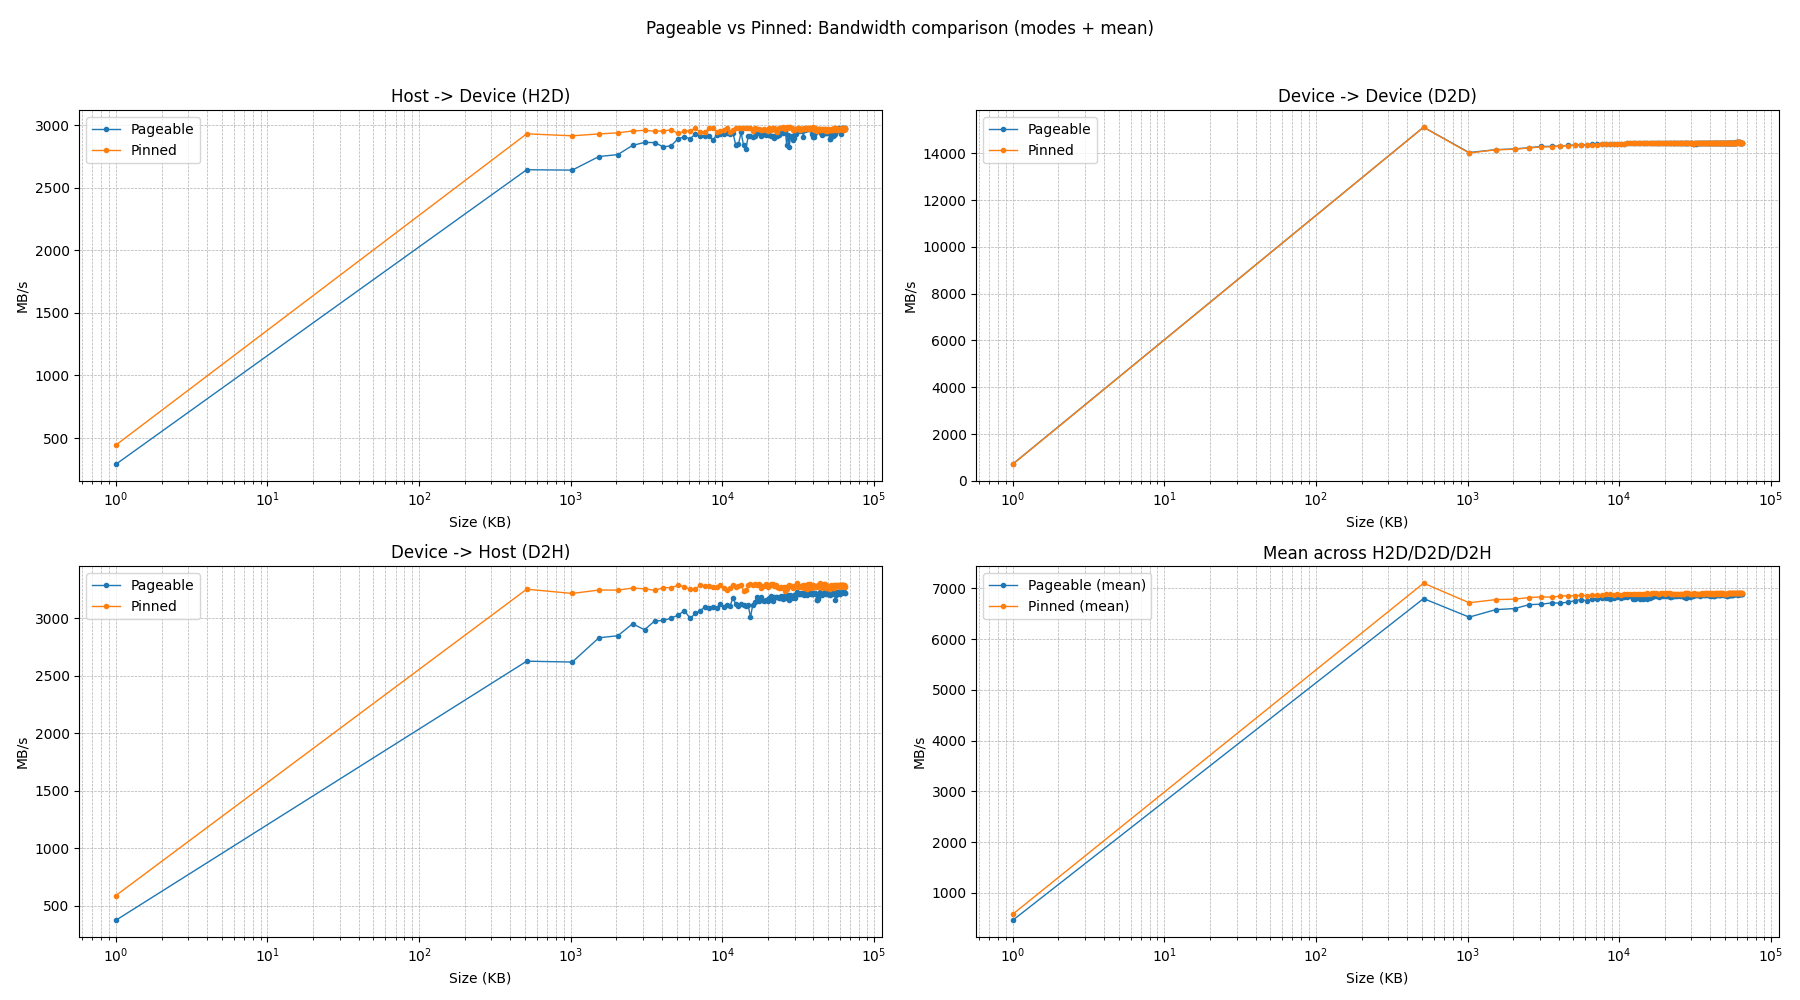
\includegraphics[width=\linewidth]{../Codigo/bandwidthTest/grafica_pageable_vs_pinned_combined.png}
        \caption{Comparativa global: Paginada vs. Bloqueada.}
    \end{subfigure}\hfill
    \begin{subfigure}[b]{0.48\textwidth}
        \centering
        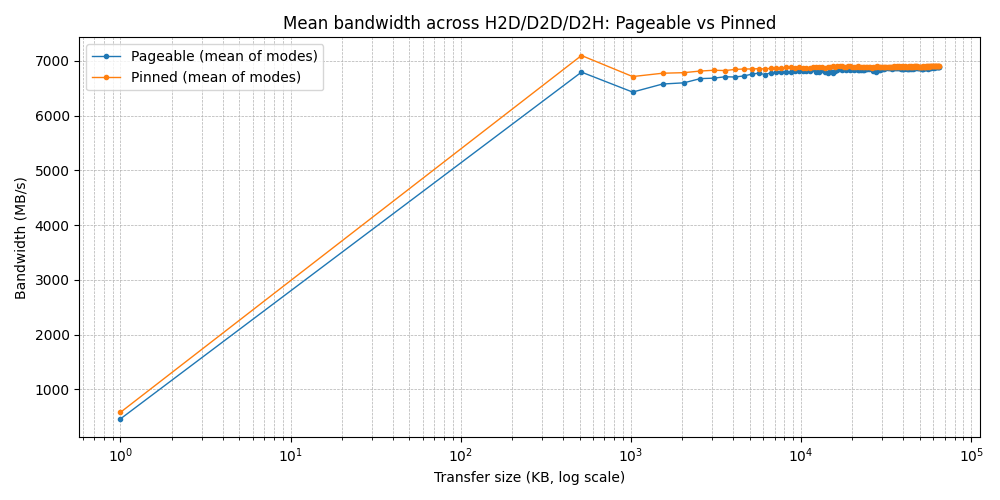
\includegraphics[width=\linewidth]{../Codigo/bandwidthTest/grafica_mean_all_types.png}
        \caption{Medias globales por tipo de transferencia.}
    \end{subfigure}
    \caption{Resumen del análisis de rendimiento de memoria.}
    \label{fig:bw_global}
\end{figure}

\begin{figure}[H]
    \centering
    \begin{subfigure}[b]{0.48\textwidth}
        \centering
        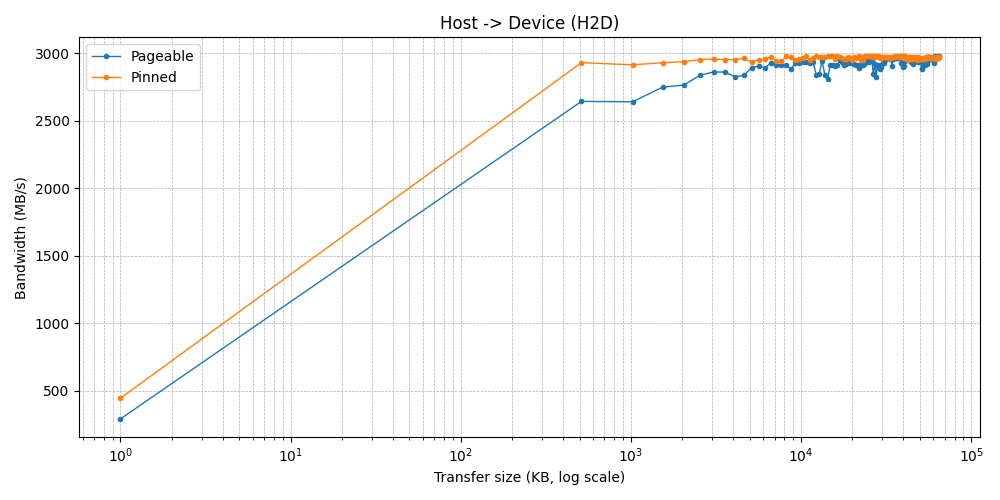
\includegraphics[width=\linewidth]{../Codigo/bandwidthTest/grafica_h2d_mb_s.png}
        \caption{Host $\rightarrow$ Device (H2D)}
    \end{subfigure}\hfill
    \begin{subfigure}[b]{0.48\textwidth}
        \centering
        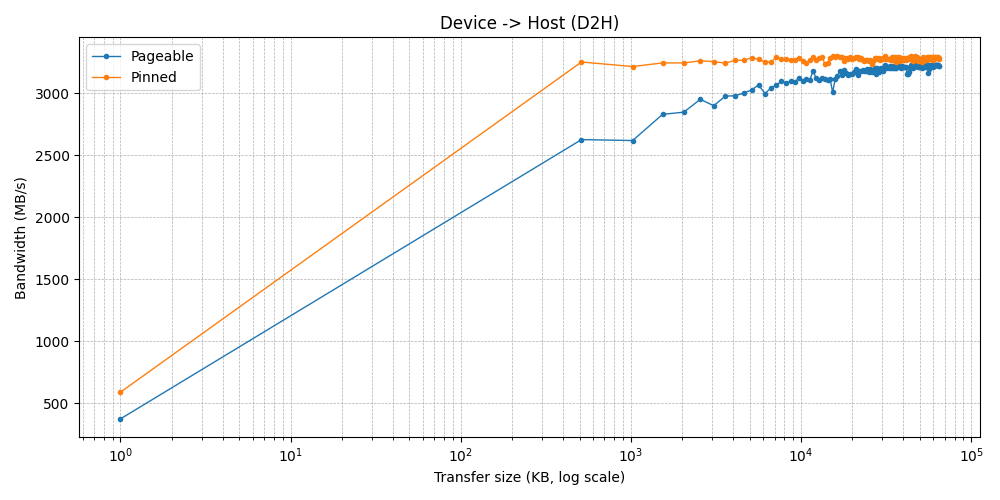
\includegraphics[width=\linewidth]{../Codigo/bandwidthTest/grafica_dtoh_mb_s.png}
        \caption{Device $\rightarrow$ Host (D2H)}
    \end{subfigure}
    \begin{subfigure}[b]{0.48\textwidth}
        \centering
        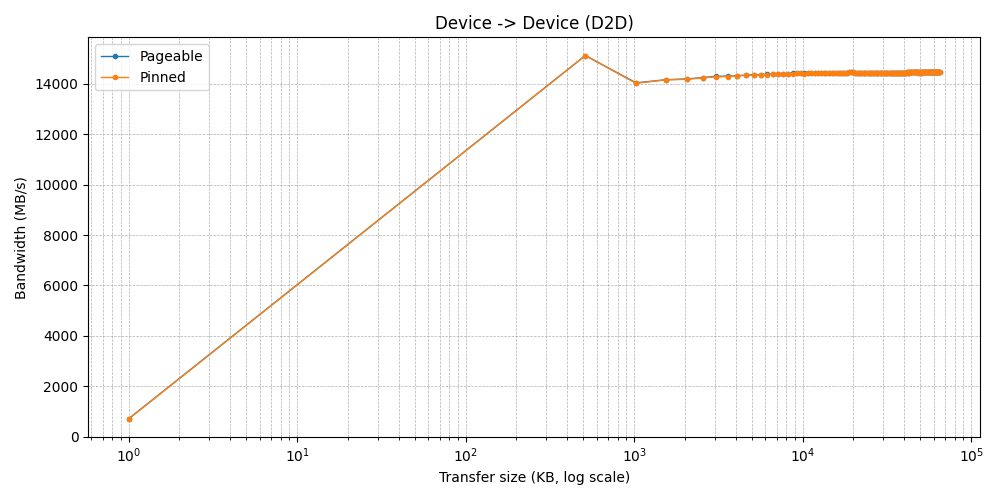
\includegraphics[width=\linewidth]{../Codigo/bandwidthTest/grafica_dtod_mb_s.png}
        \caption{Device $\rightarrow$ Device (D2D)}
    \end{subfigure}
    \caption{Detalle de ancho de banda por dirección de transferencia.}
    \label{fig:bw_detail}
\end{figure}

\subsection{Análisis cuantitativo}
La Tabla \ref{tab:bandwidth} muestra los valores medios de ancho de banda obtenidos.

\begin{table}[H]
\centering
\caption{Comparativa de ancho de banda medio (MB/s)}
\label{tab:bandwidth}
\begin{tabular}{l r r r}
    \toprule
    \textbf{Tipo} & \textbf{Pageable} & \textbf{Pinned} & \textbf{Ganancia (Speedup)} \\
    \midrule
    H2D (Host a Device) & 2901.34 & 2945.55 & 1.015$\times$ \\
    D2D (Device a Device) & 14324.27 & 14322.58 & 1.000$\times$ \\
    D2H (Device a Host) & 3136.82 & 3254.65 & 1.038$\times$ \\
    \bottomrule
\end{tabular}
\end{table}

\subsection{Discusión}
Los resultados corroboran las ventajas arquitectónicas del uso de memoria \textit{pinned}:
\begin{itemize}
    \item \textbf{Transferencias Host-Device:} Se observa una mejora en H2D y D2H. Al usar memoria bloqueada, el sistema operativo garantiza que las páginas residen en la memoria física (no se intercambian a disco), permitiendo que el motor DMA de la GPU acceda directamente a la memoria del Host. Esto elimina la necesidad de que la CPU copie los datos a un buffer intermedio del driver, reduciendo latencia y carga de CPU.
    \item \textbf{Device-Device:} Como era esperado, el tipo de memoria en el Host es irrelevante para copias internas en la VRAM de la GPU, obteniéndose resultados idénticos.
    \item \textbf{Asimetría:} Existe un rendimiento ligeramente superior en lecturas (D2H) frente a escrituras (H2D), con una ganancia máxima del 3.8\% al usar memoria \textit{pinned} en sentido D2H.
\end{itemize}

\section{Cuestión 3: Análisis del programa \texttt{cudaTemplate}}

\subsection{3.a) Funcionalidad y lógica del kernel}
El kernel \texttt{foo} implementa un patrón de acceso diseñado para ilustrar la gestión manual de la jerarquía de memoria. Las operaciones por hilo son:

\begin{enumerate}
    \item \textbf{Cálculo de índices (Linealización):} Se transforman las coordenadas del hilo a índices lineales. Primero se obtiene el índice local dentro del bloque ($tid_b$) y posteriormente el índice global ($tid_g$), considerando la geometría de la rejilla.
    \item \textbf{Carga a memoria compartida:} Cada hilo transfiere un elemento desde la memoria global (\texttt{gid\_d}) hacia su posición en la memoria compartida (\texttt{shared\_mem}).
    \item \textbf{Cómputo local:} Se actualiza el valor en memoria compartida sumando el índice global y un valor recuperado de la memoria constante (\texttt{const\_d}).
    \item \textbf{Escritura de resultados:} El valor procesado se escribe de vuelta en la memoria global.
\end{enumerate}

\subsection{3.b) Gestión de memoria compartida}
La memoria compartida se asigna dinámicamente al lanzar el kernel. El tamaño necesario es:
\[ \text{shared\_mem\_size} = \text{block.x} \times \text{block.y} \times \text{block.z} \times \text{sizeof(int)} \]

Para garantizar que esta solicitud no exceda los 49152 bytes disponibles por bloque en la GT 1030, se proponen dos validaciones:

\subsubsection*{Validación Estática}
Se actualizó la constante en \texttt{cudaTemplate.cu}: \texttt{\#define SH\_MEM\_SIZE (48 * 1024)}. Esto ajusta la aserción a los límites reales de la arquitectura Pascal.

\subsubsection*{Validación Dinámica (Recomendada)}
Para mayor portabilidad, se puede consultar el límite en tiempo de ejecución:

\begin{lstlisting}[language=C,caption={Validación dinámica de recursos}]
/*
cudaDeviceProp deviceProp;
checkCudaErrors(cudaGetDeviceProperties(&deviceProp, 0));
if (shared_mem_size > deviceProp.sharedMemPerBlock) {
    fprintf(stderr, "Error: Memoria compartida excede el limite (%zu)\n", 
            deviceProp.sharedMemPerBlock);
    exit(EXIT_FAILURE);
}
*/
\end{lstlisting}

\subsection{3.c) Sincronización}
En este diseño, existe una correspondencia uno a uno entre hilos y posiciones de memoria compartida. Dado que ningún hilo lee datos escritos por otro hilo (ausencia de dependencias cruzadas), no hay riesgo de condiciones de carrera. Por tanto, las barreras \texttt{\_\_syncthreads()} son redundantes y podrían eliminarse para optimizar el rendimiento.

\subsection{3.d) Soporte para bloques tridimensionales}
Se refactorizó el código para soportar coordenadas 3D. Las fórmulas clave implementadas para la dimensión $z$ son:

\begin{itemize}
    \item \textbf{Tamaño del bloque:} $blockSize = D_x \cdot D_y \cdot D_z$
    \item \textbf{Índice local ($tid_b$):} $tid_b = threadIdx.z \cdot (D_y \cdot D_x) + threadIdx.y \cdot D_x + threadIdx.x$
    \item \textbf{ID de bloque ($blockId$):} $blockId = blockIdx.z \cdot (G_x \cdot G_y) + blockIdx.y \cdot G_x + blockIdx.x$
\end{itemize}

Esto habilita ejecuciones volumétricas como:
\begin{lstlisting}[language=bash]
./cudaTemplate --gsx=4 --gsy=2 --gsz=2 --bsx=8 --bsy=8 --bsz=1
\end{lstlisting}

\chapter{Cuestión 4: Análisis de Rendimiento en Suma de Vectores}

En esta sección se analiza la ejecución del programa \texttt{vectorAdd}, variando el número de elementos del vector y la configuración de hilos por bloque (\texttt{tpb}). Los datos provienen de los archivos de log ubicados en \texttt{Codigo/vectorAdd}.

\section{4.a) Tiempos de ejecución y escalabilidad}

La Tabla \ref{tab:vectoradd_times} resume los tiempos medios y la desviación estándar tras 5 repeticiones por configuración.

\begin{table}[H]
\centering
\caption{Tiempos de ejecución (ms) para distintas configuraciones de \texttt{nelem} y \texttt{tpb}}
\label{tab:vectoradd_times}
\begin{tabular}{l r r}
    \toprule
    \textbf{Configuración (Elementos / TPB)} & \textbf{Media (ms)} & \textbf{Std (ms)} \\
    \midrule
    \multicolumn{3}{l}{\textit{Tamaño pequeño: 1.000.000 elementos}} \\
    1M / 128  & 5.5336 & 0.0603 \\
    1M / 256  & 5.5377 & 0.0174 \\
    1M / 1024 & 5.5785 & 0.0641 \\
    1M / 32   & 6.0064 & 1.0581 \\
    1M / 512  & 6.7275 & 2.5834 \\
    \midrule
    \multicolumn{3}{l}{\textit{Tamaño medio: 10.000.000 elementos}} \\
    10M / 128  & 49.5668 & 0.3714 \\
    10M / 256  & 49.7347 & 0.2984 \\
    10M / 512  & 49.8106 & 0.4867 \\
    10M / 1024 & 51.7977 & 4.3757 \\
    10M / 32   & 55.0660 & 11.3435 \\
    \midrule
    \multicolumn{3}{l}{\textit{Tamaño grande: 50.000.000 elementos}} \\
    50M / 1024 & 244.1822 & 0.6611 \\
    50M / 256  & 244.2601 & 0.3637 \\
    50M / 32   & 245.3972 & 0.6971 \\
    \bottomrule
\end{tabular}
\end{table}

\subsubsection*{Análisis de resultados}
\begin{itemize}
    \item \textbf{Configuraciones óptimas:} Para cargas medias (10M), los tamaños de bloque intermedios (128 y 256 hilos) ofrecen el mejor rendimiento y estabilidad.
    \item \textbf{Penalización por bloques pequeños:} El uso de \texttt{tpb}=32 resulta consistentemente más lento y presenta una desviación estándar alta. Esto se debe a una baja ocupación del hardware y un mayor overhead en la gestión de un número excesivo de bloques pequeños.
    \item \textbf{Saturación en bloques grandes:} Para 50M de elementos, las diferencias entre 256 y 1024 hilos se diluyen, indicando que el cuello de botella se desplaza hacia el ancho de banda de memoria global más que hacia la capacidad de cómputo.
\end{itemize}

\section{4.b) Implementación del Kernel}

El código del kernel (\texttt{vectorAdd\_kernel.cu}):

\begin{lstlisting}[language=C,caption={Kernel \texttt{vectorAdd}}]
__global__ void vectorAdd(const float *X, const float *Y, float *V, int numElements)
{
    int tid = blockDim.x * blockIdx.x + threadIdx.x;
    if (tid < numElements) {
        V[tid] = X[tid] + Y[tid];
    }
}
\end{lstlisting}

En el, cada hilo calcula un identificador único global (\texttt{tid}). La condición \texttt{if (tid < numElements)} es crítica para evitar accesos ilegales a memoria cuando el número total de hilos lanzados excede el tamaño del vector.

\section{4.c) Dimensionamiento del Grid}

El número de bloques necesarios se calcula en el Host mediante la fórmula de redondeo hacia arriba:
\begin{equation}
    blocksPerGrid = \left\lceil \frac{numElements}{threadsPerBlock} \right\rceil = \frac{numElements + threadsPerBlock - 1}{threadsPerBlock}
\end{equation}

Esta estrategia asegura que se generen suficientes hilos para cubrir todos los elementos del vector. Cuando $numElements$ no es múltiplo de $threadsPerBlock$, el último bloque contendrá hilos "inactivos" (cuyo $tid \ge numElements$), los cuales serán descartados por el condicional dentro del kernel, garantizando la corrección del programa.

\section{4.d) Influencia del Warp en el Rendimiento}

El \textbf{warp} es la unidad fundamental de despacho de instrucciones en la arquitectura CUDA, constituida por 32 hilos que se ejecutan en modo SIMT (\textit{Single Instruction, Multiple Threads}). La alineación con el tamaño del warp es crucial por tres motivos:

\begin{enumerate}
    \item \textbf{Subutilización (Underutilization):} Si el tamaño del bloque no es múltiplo de 32, el último warp del bloque estará parcialmente vacío. Los hilos inexistentes ocupan "slots" de ejecución sin realizar trabajo útil, desperdiciando ciclos de computación.
    \item \textbf{Divergencia de ramas:} Aunque no aplica en este kernel simple, en algoritmos complejos, si los hilos de un mismo warp toman caminos distintos en un condicional, la ejecución se serializa, degradando el rendimiento.
    \item \textbf{Coalescencia de memoria:} El hardware de memoria está optimizado para servir peticiones de 32 hilos consecutivos simultáneamente. Si los bloques o los accesos no están alineados, se requieren más transacciones de memoria para servir la misma cantidad de datos.
\end{enumerate}

Los resultados empíricos (Tabla \ref{tab:vectoradd_times}) donde \texttt{tpb}=32 muestra peor rendimiento y alta variabilidad, confirman que tamaños de bloque muy reducidos impiden ocultar eficazmente la latencia de memoria y aumentan la sobrecarga de planificación de warps.

\end{document}